%!TEX root=Projektdokumentation_ClockPendulumAnalyzer.tex
\section{Ausblick}
Der vorliegende Prototyp eines \documenttitle\ bietet eine Grundlage, um diverse Arten von Uhrenpendel auf einige Mikrosekunden genau auszumessen. Die Genauigkeit ist hauptsächlich durch den Sensor und den Referenzkristall gegeben, die übrigen Systemelemente arbeiten konstant, dies bedeutet, der Zeitbedarf ist immer gleich und somit hebt sich dies zwischen zwei Messungen auf.\\
Das System kann somit mit den folgenden Massnahmen optimiert werden:
\begin{itemize}
	\item Ersatz des eingebauten Kristalls des tiny K20 Mikrocontroller-Boards durch einen externen, hochgenauen Kristall, z.B. einem NH25M22TA der Firma NDK. Mit einer Abweichung von 0.003ppm der 3ppb\footnote{Parts per Billion} und einer Spannung von 3.3V lässt er sich direkt an das tiny K20 anschliessen und würde auch im Gehäuse noch Platz finden. Nachteil ist der Stückpreis von ca. 85.- Franken bei einem Stück. Mit 10MHz eignet sich die Frequenz, um den Flankenzähler des tiny K20 zu speisen. Das Datenblatt befindet sich im Anhang ab Seite \pageref{app:NH25M22TA}.
	\item Verwenden eines anderen Sensors. Beispielsweise eine Laserschranke anstelle einer Infrarot-Schranke mit entsprechend weniger Streuung dank dem dünneren Laserstrahl. Allerdings konnte während der Recherchephase keine geeignete Laserschranke gefunden werden, welche keinen Empfänger benötigt.
	\item Einsatz eines leistungsstärkeren Mikrocontroller-Systems. Aktuell werden an der Hochschule Luzern Technik \& Architektur die ersten Modelle des neuen tiny K22 hergestellt. Dieses neue Board weist gegenüber dem kleineren K20 folgende Vorteile auf und ist ebenfalls für ca. 20.- Franken erhältlich (Abbildung \ref{fig:tinyk22-overview}, mcuoneclipse.com):
	\begin{itemize}
		\item 160Mhz Prozessor, Freescale K22
		\item 512 KByte FLASH und 128 KByte RAM.
		\item Grössere Anzahl I/O Ports.
		\item Eigener Freescale K20 Prozessor und USB Port zum Debuggen. 
	\end{itemize}
	Allerdings weist das tiny K22 andere Footer auf, so dass das \hwb\ entsprechend neu gestaltet werden müsste.
	\item Vollumfänglicher Einsatz der RTC zusammen mit dem GPS-Modul: Die RTC könnte als eigener Zeitgeber genutzt werden, wenn kein NTP-Server verfügbar ist. Die entsprechenden \iic Anschlüsse sind auf dem \hwb\ vorhanden. Mit Hilfe des GPS-Moduls kann die aktuelle Umgebungszeit über UART-RS232 gesetzt werden. Diese Anschlüsse sind ebenfalls bereits vorbereitet.  
\end{itemize}
\begin{figure}[H]
	\centering
	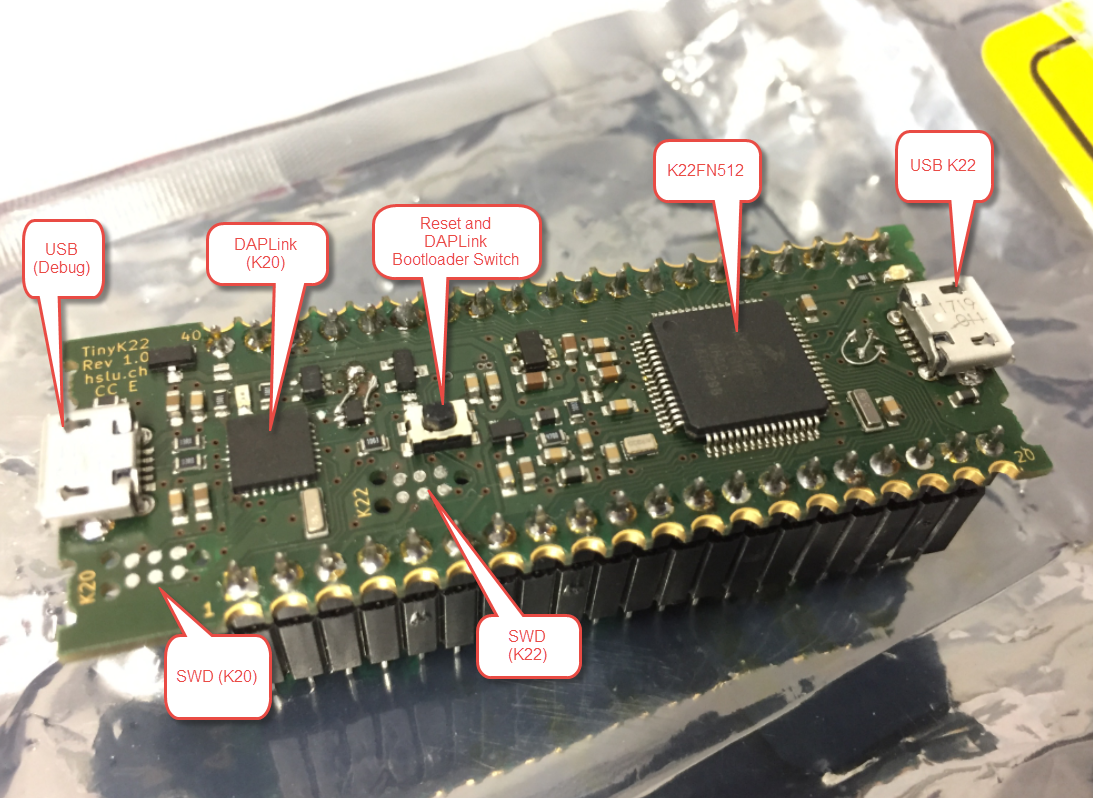
\includegraphics[width=0.5\textwidth]{tinyk22-overview}
	\caption{Tiny K22 Board mit eigenem Debug- Anschluss (Bildquelle: mcuoneclipse.com)}
	\label{fig:tinyk22-overview}
\end{figure}
Aktuell ist die Zähler-Frequenz von 12MHz in allen Softwareteilen fest eingetragen. Entsprechend müsste diese bei einer Änderung angepasst werden. Optimalerweise kann das System so erweitert werden, dass die Frequenz über ein Konfigurations-File eingestellt werden kann oder vom Mikrocontroller- System gleich automatisch ermittelt und gesetzt wird.\\
Allerdings bedingt der Einsatz eines externen Zählers ebenfalls Änderungen an der Software und es ist kaum anzunehmen, dass sich die Zählerfrequenz laufend ändert.